\documentclass[article]{jss}
\usepackage[T1]{fontenc}
\usepackage[utf8]{inputenc}
\usepackage{booktabs}
\usepackage{longtable}

\usepackage{amsmath}

\usepackage{natbib}
\usepackage[a4paper]{geometry}
\usepackage{color}
\usepackage{rotating}
\usepackage{graphicx}
\usepackage[noprefix]{nomencl}
\usepackage{subfig}
\usepackage{hyperref}



\author{Fernando Antonanzas-Torres\\Universidad de La Rioja \And
F. Javier Martínez-de-Pisón\\Universidad de La Rioja \AND
Javier Antonanzas \\Universidad de La Rioja \And 
Oscar Perpiñán\\ Universidad Politecnica de Madrid}
\title{Downscaling of solar irradiation in \proglang{R}}


\Plainauthor{Fernando Antonanzas-Torres, Javier Martinez-de-Pison, Javier Antonanzas, Oscar Perpinan} 
\Plaintitle{Downscaling of solar irradiation in R} 

\Abstract{
 A methodology to downscale solar irradiation from
    satellite-derived databases is described using \proglang{R}
    software. Different packages such as \pkg{raster},
    \pkg{parallel}, \pkg{solaR}, \pkg{gstat}, \pkg{sp}
    and \pkg{rasterVis} are considered in this study to improve
    solar resource estimation in areas with complex topography, in
    which the downscaling suppose a very useful tool to reduce
    inherent deviations of satellite-derived irradiation
    databases, which globally lack of high spatial resolution. A
    topographical analysis of horizon blocking and sky-view is
    developed with a digital elevation model to determine which
    fraction of hourly solar irradiation reaches the Earth
    surface. Eventually, \emph{kriging with external drift} is
    applied for a better estimation of solar irradiation
    throughout the region analyzed. This methodology has been
    implemented as an example within La Rioja region in northern
    Spain, highlighting a mean absolute error 14\% lower than
    with the original database. 
}
\Keywords{solar  irradiation, \proglang{R}, \pkg{raster}, \pkg{solaR}, digital elevation model, shade analysis, downscaling}
\Plainkeywords{solar  irradiation, R, raster, solaR, digital elevation model, shade analysis, downscaling} 



\Address{
Oscar Perpiñán Lamigueiro\\
Departamento de Ingeniería Eléctrica\\
Universidad Politécnica de Madrid\\
Madrid, Spain\\
E-mail: \email{oscar.perpinan@gmail.com}\\
URL: \url{http://procomun.wordpress.com}
}




\begin{document}


\section{Introduction}

During the last few years the development of photovoltaic energy has
flourished in developing countries with both multi-megawatt power
plants and micro installations. However, the scarcity of long and
reliable solar irradiation data from pyranometers in many of these
countries makes necessary the estimation of solar irradiation from
other meteorological variables or satellite photographies
\cite{Schulz.Albert.ea2009}. In the case of estimating irradiation
from other measured meteorological variables, models need to be
validated with nearby pyranometer registers, since these models lack
of spatial generalization.

Thus, in some regions without any nearby pyranometer these models
become not an option and therefore, irradiation data must be obtained
from satellite estimates. Although satellite-derived irradiation
databases such as the NASA Surface meteorology and Solar Energy
(SSE)\footnote{\url{http://maps.nrel.gov/SWERA}}, the National
Renewable Energy Laboratory
(NREL)\footnote{\url{http://www.nrel.gov/gis/solar.html}},
INPE\footnote{\url{http://www.inpe.br}},
SODA\footnote{\url{http://www.soda-is.com/eng/index.html}} and the
Climate Monitoring Satellite Application Facility (CM
SAF)\footnote{\url{http://www.cmsaf.eu}} provide wide spatial
coverage, only NASA and some CM SAF climate data sets present global
coverage, while diminishing its spatial resolution
(Table~\ref{tab:databases}).

\begin{small}
\begin{longtable}{p{0.12\textwidth}p{0.16\textwidth}p{0.16\textwidth}p{0.10\textwidth}p{0.12\textwidth}p{0.12\textwidth}}
  \toprule
\ Database&Product&Spatial coverage&Spatial resolution&Temporal coverage&Temporal resolution \\
\midrule
\endhead
CM SAF&SIS Climate Data Set (GHI)&Global&0.25x0.25$^\circ$&1982-2009&Daily means\\
\midrule
CM SAF&SIS Climate Data Set (GHI)&70S-70N, 70W-70E&0.03x0.03$^\circ$&1983-2005&Hourly means\\
\midrule
CM SAF&SID Climate Data Set (BHI)&70S-70N, 70W-70E&0.03x0.03$^\circ$&1983-2005&Hourly means\\
\midrule
SODA& Helioclim 3 v2 and v3 (GHI)&66S-66N,66W-66E&~5km&2005&15 minutes\\
\midrule
SODA& Helioclim 3 v2 and v3 (GHI)&66S-66N,66W-66E&~5km&2005&15 minutes\\
\midrule
NREL& GHI Moderate resolution&Central and South America, Africa, India, East Asia&40x40km&1985-1991&Monthly means of daily GHI\\
\midrule
NASA& SSE&Global&1x1$^\circ$&1983-2005&Daily means\\
\bottomrule
\caption{Summary of solar irradiation databases}
  \label{tab:databases}
\end{longtable}
\end{small}


The spatial resolutions of satellite estimates are generally in the
range of kilometers, averaging solar irradiation and omitting the
impact of topography within each cell. As a result, intra-cell
variations can be very significative in areas with local
micro-climatic characteristics and also in areas with complex
topography, which in many occasions coincide. Thus, under these events
these irradiation data might not be of sufficient accuracy to project
a photovoltaic installation. \citep{Perez.Seals.ea1994} analyzed the
spatial behavior of solar irradiation and concluded that the
break-even distance from satellite estimates against pyranometers is
in the order of 7 km and that variations are harsh to be estimated for
distances further than 40
km. \cite{Antonanzas-Torres.Canizares.ea2013} rejected ordinary
kriging as a spatial interpolation method of solar irradiation in
Spain with stations separated more than 50 km in mountainous regions,
as a result of its high spatial variability in these areas. The
NASA-SSE and CM SAF SIS Climate Data Set (GHI) provide global coverage
with resolutions of 1x1$^\circ$ and 0.25x0.25$^\circ$
(Table~\ref{tab:databases}), which in most latitudes implies a grosser
resolution than the previously mentioned 40-50 km.  One of the
alternatives to obtain higher spatial resolution of solar irradiation
is the downscaling of satellite-estimates. Irradiation downscaling can
be based on interpolation kriging techniques when pyranometers
registers are available, implementing related-to-irradiation
continuous variables such as elevation, sky-view-factor and other
meteorological variables as external drifts
\citep{Alsamamra.Ruiz-Arias.ea2009} \citep{Batlles.Bosch.ea2008}. The
downscaling is generally based on digital elevation models (DEM) with
satellite-derived irradiation data to account for the effect of
complex topography and has been previously applied in mountainous
areas such as the Mont Blanc Massif (France) \citep{Corripio2003} and
Sierra Nevada (Spain) \citep{Bosch.Batlles.ea2010} \citep{Ruiz-Arias.Cebecauer.ea2010} with image resolutions of
3.5x3.5 km.  However, the NASA-SSE and CM SAF SIS Climate Data Set
are based on much lower resolutions and suppose the unique irradiation
datasets in numerous countries recently interested in solar energy.

In this paper, a downscaling methodology of global solar
irradiation is explained by means of \proglang{R}-Project software
and studied over La Rioja region (very mountainous region in
northern Spain). Data from the CM SAF with 0.03x0.03$^\circ$
resolution is considered and then downscaled to higher resolution
(200x200m). On a second step, \emph{kriging with external
  drift}, also denoted as \emph{universal kriging}, is applied to
interpolate data from 6 on-ground pyranometers within the region
considering this downscaled CM SAF data as explanatory
variable. Eventually, a downscaled map of annual global solar
radiation is obtained throughout this region.




\section{Data}

The CM SAF was funded in 1992 as a joint venture of several
European meteorological institutes, with the collaboration of the
European Organization for the Exploitation of Meteorological
Satellites (EUMETSAT) to retrieve, archive and distribute climate
data to be used for climate monitoring and climate analysis
\citep{Posselt.Mueller.ea2012a}. Two kind of categories
are provided: operational products and climate data. The
operational products are built on data validated with on-ground
stations and provided in near-to-present time and the climate data
are long-term series to evaluate inter-annual variability.

This study is built on hourly surface incoming solar radiation and
direct irradiation climate data, denoted as SIS and SID by CM SAF
respectively, for the year 2005. These climate data have been
derived from Meteosat first generation satellites (Meteosat 2 to
7, 1982-2005) and validated using on-ground registers from the
Baseline Surface Radiation Network (BSRN) as a reference. The
target accuracy of SIS and SID in hourly means is 15 $W/m^{2}$
\citep{Posselt.Muller.ea2011}, providing a maximum spatial resolution of
0.03x0.03$^\circ$. In the study, SIS and SID data are selected with
spatial resolution of 0.03x0.03$^\circ$. Data is freely accesible via
FTP through the CM SAF website.

Hourly GHI registers from SOS
Rioja\footnote{\url{http://www.larioja.org/npRioja/default/defaultpage.jsp?idtab=442821}}
in 6 meteorological stations (shown in
Figure~\ref{fig:mapstations} and Table~\ref{tab:stations}) during
2005 serve as complementary measurements for the downscaling
within the region studied.

\begin{figure}[H]
  \centering
  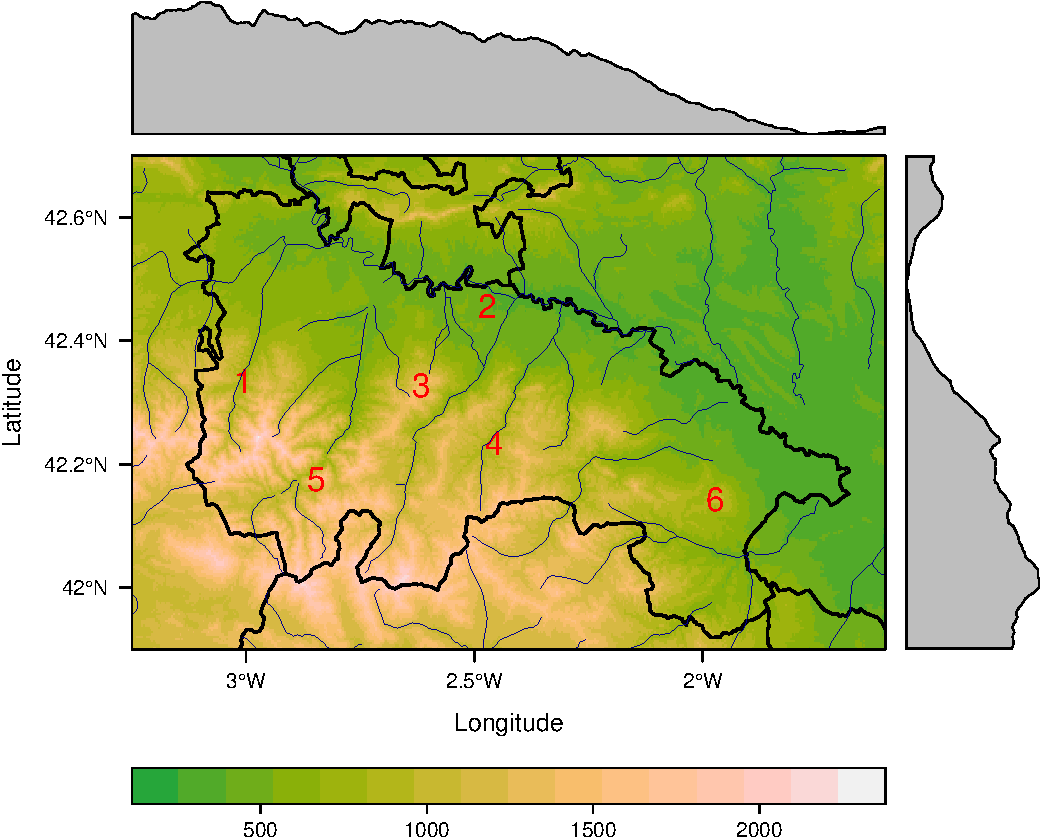
\includegraphics[width=\textwidth]{figs/mapstations.pdf}
  \caption{Region analyzed and meteorological stations considered}
  \label{fig:mapstations}
\end{figure}

These stations integrate First Class pyranometers (according to ISO
9060) with uncertainty of 5\% in daily totals. These data have been
filtered from spurious assuming in those cases the average between the
previous and following hourly measurements.

The digital elevation model (DEM) is obtained from the product
MDT-200 of the \copyright Spanish Institute of
Geography\footnote{\url{http://www.ign.es}} with spatial
resolution of 200x200m.


\begin{small}
\begin{longtable}{p{0.01\textwidth}p{0.12\textwidth}p{0.06\textwidth}p{0.05\textwidth}p{0.06\textwidth}p{0.05\textwidth}p{0.05\textwidth}}
  \toprule
  \# & Name & Net. & Lat.(º) & Long.(º) & Alt.  & $GHI_{a}$\\
  \midrule
  \endhead
 1 & Ezcaray & SOS & 42.33 & -3.00 & 1000 & 1479\\
  \midrule
 2 & Logroño & SOS & 42.45 & -2.74 & 408 & 1504\\
  \midrule 
3 & Moncalvillo & SOS & 42.32 & -2.61 & 1495 & 1329 \\
  \midrule
 4 & San Roman & SOS & 42.23 & -2.45 & 1094 & 1504 \\
  \midrule
  5 & Ventrosa & SOS & 42.17 & -2.84 & 1565 & 1277\\
  \midrule
  6 & Yerga & SOS& 42.14 & -1.97 & 1235 &1448\\
 \bottomrule
  \caption{Summary of the meteorological
    stations selected.}
  \label{tab:stations}
\end{longtable}
\end{small}

\section{Method}
\label{sec:method}

This section describes the methodology
proposed. Figure~\ref{fig:method} displays the method diagram using
red ellipses and lines for data sources, blue ellipses and lines for
derived rasters (results), and black rectangles and lines for
operations.
\begin{figure}
  \centering
  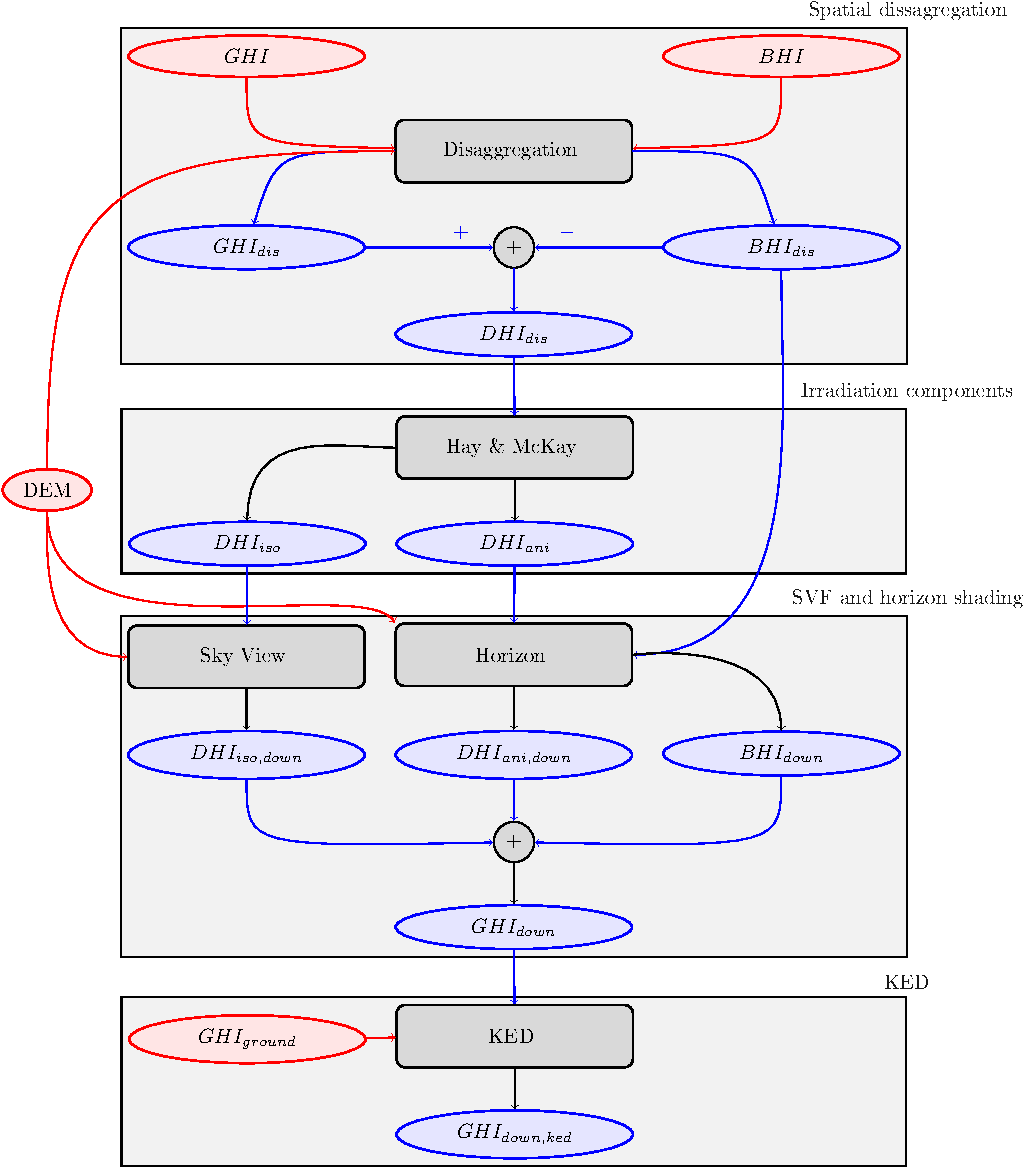
\includegraphics[width=\textwidth]{figs/algorithmScheme.pdf}
  \caption{Methodology of downscaling: this figure uses red ellipses
    and lines for data sources, blue ellipses and lines for derived
    rasters (results), and black rectangles and lines for operations.
  }
  \label{fig:method}
\end{figure}


\subsection{Irradiation decomposition}
\label{sec:irradDecomp}

Initially, diffuse horizontal irradiation ($DHI$) is obtained
throughout the difference between global horizontal irradiation
($GHI$) and beam horizontal irradiation ($BHI$) rasters,
previously obtained from CM SAF.


$DHI$ and $BHI$ are firstly disaggregated from the original gross
resolution (0.03x0.03$^\circ$) into the DEM resolution (200x200m),
leading to remain similar values in disaggregated pixels to the
original gross resolution pixel.

On a second step, $DHI$ can be divided in two components:
isotropic diffuse irradiation ($DHI_{iso}$) and anisotropic
diffuse irradiation ($DHI_{ani}$) according to the Hay \& Mckay
model \citep{Hay.Mckay1985} (Equation~\ref{eq:DHI}). This model is
based on the anisotropy index ($k_{1}$) defined as the relation
between the beam irradiance ($B(0)$) and the extra-terrestrial
irradiance ($B_{0}(0)$), as shown in Equation~\ref{eq:k1}. High
$k_{1}$ values are typical in clear sky atmospheres, while low
$k_{1}$ values are frequent in overcasted and atmospheres with high
aerosol density.


\begin{equation}
  \label{eq:DHI}
  DHI=DHI_{iso}+DHI_{ani}
\end{equation}

\begin{equation}
  \label{eq:k1}
  k_{1}=\frac{B(0)}{B_{0}(0)} 
\end{equation}

The $DHI_{iso}$ accounts for the incoming diffuse irradiation
portion from an isotropic sky, being more significant in very
cloudy days (Equation~\ref{eq:DHIisos}).

\begin{equation}
  \label{eq:DHIisos}
  DHI_{iso}=DHI\cdot{}(1-k_{1})
\end{equation}

$DHI_{ani}$, also denoted as circumsolar diffuse irradiation,
considers the incoming portion from the circumsolar disk and can be
analyzed as beam irradiation \citep{Perpinan-Lamigueiro2012a}
(Equation ~\ref{eq:DHIani}).

\begin{equation}
  \label{eq:DHIani}
  DHI_{ani}=DHI\cdot{}k_{1}
\end{equation}


\subsection{Sky view factor and horizon blocking}
\label{sec:sky-view-factor}

The topographical analysis is performed accounting for the visible
sky sphere (sky view) and also the horizon blocking. The
$DHI_{iso}$ is directly dependent on the sky-view factor (SVF),
which computes the proportion of visible sky related to a flat
horizon. The sky-view factor has been previously considered in
other irradiation assessments \citep{Ruiz-Arias.Cebecauer.ea2010, Corripio2003}. The sky view factor is calculated in each DEM
pixel considering 72 vectors (separated 5$^\circ$ each) and evaluating
the maximum horizon angle ($\theta_{hor}$) along 20km in each
vector (Equation~\ref{eq:SVF}). The $\theta_{hor}$ stands for the
maximum angle between the altitude of a location and the elevation
of the group of points along each vector, related to a horizontal
plane on the location. Locations without horizon blocking achieve
SVF close to 1, which stands for a whole visible sky semi-sphere.

\begin{equation}
  \label{eq:SVF}
  SVF=1-\int_0^{2\pi}sin^{2} \theta_{hor} \delta \theta
\end{equation}

Eventually, the downscaled $DHI_{iso}$ ($DHI_{iso,down}$) is
computed with Equation~\ref{eq:DHIiso}.

\begin{equation}
  \label{eq:DHIiso}
  DHI_{iso,down}=DHI_{iso}\cdot{}SVF
\end{equation}

The horizon blocking is analyzed evaluating the solar geometry in
15 minutes samples, particularly the solar elevation
($\gamma_{s}$) and the solar azimuth ($\psi_{s}$). Secondly, the
mean hourly $\gamma_{s}$ and $\psi_{s}$ (from those 15 minutes
rasters) are calculated and then disaggregated as previously
explained for $DHI$ and $BHI$ rasters. The decision of solving the
solar geometry with low resolution rasters permits reducing
significantly computational time without penalizing results.

The $\theta_{hor}$ corresponding to each $\psi_{s}$ is compared
with the $\theta_{zs}$. As a consequence, if the $\theta_{zs}$ is
greater than the $\theta_{hor}$ implies horizon blocking on the
surface analyzed and therefore, $BHI$ and $DHI_{ani}$
blocked. Eventually, the sum of $DHI_{ani,down}$, $DHI_{iso,down}$
and $BHI_{iso,donw}$ constitutes the downscaled global horizontal
irradiation $GHI_{down}$.

\subsection{Post-processing: kriging with external drift}
\label{sec:meth}
The fact that the afore-explained downscaling accounts for the
irradiation loss due to the horizon blocking and sky-view factor
leads to introduce a trend in estimates (lowering them) when
compared with the original data (gross resolution data). However,
satellite-derived irradiation data is implicitly considering
shades, as a consequence of the lower albedo registered in these
zones, although it is latter averaged throughout the
pixel. $GHI_{down}$ can be considered as useful bias of the
behavior of solar irradiation within the region studied. The
\emph{universal kriging} or \emph{kriging with external drift}
(KED) includes the information from exhaustively-sampled
explanatory variables in the interpolation. As a result,
$GHI_{down}$ is considered the explanatory variable to interpolate
measured irradiation data from some on-ground calibrated
pyranometers which is denoted as
\emph{post-processing}. $GHI_{down}$ is correlated with the DEM as
a consequence of the high influence of the horizon blocking with
topography and therefore estimations can be derived separating the
deterministic ($\hat{m}(\mathbf{s}_\theta)$) and stochastic
components ($\hat{\epsilon}(\mathbf{s}_\theta)$)
(Equations~\ref{eq:externalDrift} and
~\ref{eq:externalDrift_sum}).

\begin{equation}
  \label{eq:externalDrift}
  \hat{z}(\mathbf{\mathbf{s}}_\theta) = \hat{m}(\mathbf{s}_\theta) + \hat{\epsilon}(\mathbf{s}_\theta)
\end{equation}

\begin{equation}
  \label{eq:externalDrift_sum}
  \hat{z}(\mathbf{s}_\theta) =  \sum_{k=0}^p \hat{\beta}_k q_k(\mathbf{s}_\theta) + 
  \sum_{i=1}^n \lambda_i \epsilon(\mathbf{s}_i)
\end{equation}
where $\hat{\beta}_k$ are the estimated coefficients of the
deterministic model, $q_k(\mathbf{s}_\theta)$ are the auxiliary
predictors obtained from the fitted values of the explanatory
variable at the new location, $\lambda_i$ are the kriging weights
determined by the spatial dependence structure of the residual,
and $\epsilon(\mathbf{s}_i)$ are the residual at location
$\mathbf{s}_i$ \citep{Antonanzas-Torres.Canizares.ea2013}.

The semivariogram is a function defined as
Equation~\ref{eq:variogram} based on a constant variance of
$\epsilon$ and also on the assumption that spatial correlation of
$\epsilon$ depends on the distance amongst instances
($\mathbf{h}$) instead of their position
\citep{Pebesma2004}.
\begin{equation}
  \label{eq:variogram}
  \gamma(\mathbf{h}) = \frac{1}{2} \textrm{E}(\epsilon(\mathbf{s}) -
  \epsilon(\mathbf{s} + \mathbf{h}))^2
\end{equation}

Given that the afore-explained sample variogram only collates
estimates from observed points, a fitting model of this variogram
is generally considered to extrapolate the spatial behavior of
observed points to the area studied.  In the literature different
variogram functions are commonly defined such as the exponential,
gaussian or spherical models. In this line, different parameters
such as the sill, range and nugget of the model must be adjusted
to best fit the sample variogram \citep{Hengl2009}. The nugget
effect, generally associated to intrinsec micro-variability and
measurement error, models the discontinuity of the variogram at
the origin. It must be highlighted that when the nugget effect is
recorded, kriging differs from a regular interpolation and as a
result estimates are different from measured values. The variogram
model of solar horizontal irradiation has been evaluated in Spain,
concluding that a pure nugget fitting behaves best, implying no
spatial auto-correlation on residuals
\citep{Antonanzas-Torres.Canizares.ea2013}.

\section{Implementation}
\label{sec-1}


The methodology proposed is applied in La Rioja region (north of
Spain). Figure~\ref{fig:cmsaf} shows the correspondent annual
global horizontal irradiation from CM SAF with resolution
0.03x0.03$^\circ$. 

\subsection{Packages}
\label{sec-1-1}

The downscaling described in this paper has been implemented using
the free software environment R \citep{proglangRDevelopmentCoreTeam2013}
and several contributed packages:

\begin{itemize}
\item \pkg{raster} \citep{Hijmans.Etten2013} for spatial data manipulation
  and analysis.
\item \pkg{solaR} \citep{Perpinan-Lamigueiro2012} for the solar
  geometry.
\item \pkg{gstat} \citep{Pebesma.Graeler2013} and \pkg{sp}
  \citep{Pebesma.Bivand.ea2013} for the geostatistical analysis.
\item \pkg{parallel} for multi-core parallelization.
\item \pkg{rasterVis} \citep{Perpinan-Lamiguiero.Hijmans2013} for spatial data
  visualization methods.
\end{itemize}

\begin{CodeChunk}
\begin{CodeInput}
R> library(sp)
R> library(raster)
R> rasterOptions(todisk=FALSE)
R> rasterOptions(chunksize = 1e+06, maxmemory = 1e+07)
R> library(maptools)
R> library(gstat)
R> library(lattice)
R> library(latticeExtra)
R> library(rasterVis)
R> library(solaR)
R> library(parallel)
\end{CodeInput}
\end{CodeChunk}


\subsection{Data}
\label{sec-1-2}

Satellite data can be freely downloaded previous registration from CM
SAF\footnote{\url{www.cmsaf.eu}} in the \emph{data access} space selecting \emph{web user interface} and \emph{climate data sets} and then choosing
hourly climate data sets named \emph{SIS} (Global Horizontal
Irradiation)) and \emph{SID} (Beam Horizontal Irradiation) for
2005. Both rasters are projected to the UTM projection for
compatibility with the Digital Elevation Model.


\begin{CodeChunk}
\begin{CodeInput}
R> projUTM  <-  CRS('+proj=utm +zone=30')
R> projLonLat <- CRS(' +proj=longlat +ellps=WGS84')

R> listFich <- dir(pattern='SIShm2005')
R> stackSIS <- stack(listFich)
R> stackSIS <- projectRaster(stackSIS,crs=projUTM)

R> listFich <- dir(pattern='SIDhm2005')
R> stackSID <- stack(listFich)
R> stackSID <- projectRaster(stackSID, crs=projUTM)
\end{CodeInput}
\end{CodeChunk}

We compute the annual global irradiation which will be used as the
reference for future steps.
\begin{CodeChunk}
\begin{CodeInput}
R> SISa2005 <- calc(stackSIS, sum, na.rm=TRUE)
\end{CodeInput}
\end{CodeChunk}

The Spanish Digital Elevation Model is obtained previous registration from the \copyright
Spanish Institute of Geography\footnote{\url{http://www.ign.es}} in the \emph{free download of digital geographic information for non-commercial use} space, and then
crop to the region analyzed (La Rioja). As stated above, this DEM uses
the UTM projection.

\begin{CodeChunk}
\begin{CodeInput}
R> elevSpain <- raster('elevSpain.grd')
R> elev <- crop(elevSpain, extent(479600, 616200, 4639600, 4728400))
R> names(elev)<-'elev'
\end{CodeInput}
\end{CodeChunk}

\subsection{Sun geometry}
\label{sec-1-3}

The first step is to compute the sun angles (height and azimuth)
and the extraterrestial solar irradiation for every cell of the
CMSAF rasters. The function \code{calcSol} from the \pkg{solaR}
package calculates the daily and intradaily sun geometry. This
function and the \code{overlay} method from the \pkg{raster}
package produce three multilayer \code{Raster} objects with the
sun geometry needed for the next steps. For the sake of brevity we
show only the procedure for the extraterrestial solar
irradiation. The calculation of sun geometry is performed with the
resolution of CM SAF.

As a first step, we define a function to extract the hour for
aggregation, choose the annual irradiation raster as reference, and
define a raster with longitude and latitude coordinates.
\begin{CodeChunk}
\begin{CodeInput}
R> hour <- function(tt)as.POSIXct(trunc(tt, 'hours'))

R> r <- SISa2005

R> latlon <- stack(init(r, v='y'), init(r, v='x'))
R> names(latlon) <- c('lat', 'lon')
\end{CodeInput}
\end{CodeChunk}


The extraterrestrial irradiation is calculated with 5-min
samples. Every point is a column of the \code{data.frame}
\code{locs}. Its columns are traversed with \code{lapply} so for
every point of the \code{Raster} object a time series of
extraterrestial solar irradiation is computed.  The result,
\code{B05min}, is a \code{RasterBrick} object with a layer for
each element of the time index \code{BTi}, which is aggregated to
an hourly raster with \code{zApply} and transformed to the UTM
projection.

\begin{CodeChunk}
\begin{CodeInput}
R> BTi <- seq(as.POSIXct('2005-01-01 00:00:00'),
+            as.POSIXct('2005-12-31 23:55:00'), by='5 min')

R> B05min <- overlay(latlon, fun=function(lat, lon){
+     locs <- as.data.frame(rbind(lat, lon))
+     b <- lapply(locs, function(p){
+ 
+         hh <- local2Solar(BTi, p[2])
+         sol <- calcSol(p[1], BTi=hh)
+         Bo0 <- as.data.frameI(sol)$Bo0
+         Bo0 })
+     res <- do.call(rbind, b)})

R> B05min <- setZ(B05min, BTi)
R> names(B05min) <- as.character(BTi)

R> B0h <- zApply(B05min, by=hour, fun=mean)
R> projectRaster(B0h,crs=projUTM)
\end{CodeInput}
\end{CodeChunk}

\subsection{Irradiation components}
\label{sec-1-4}

The CMSAF rasters must be transformed to the higher resolution of
the DEM (UTM 200mx200m). As a consequence of the different pixel
geometry between DEM (square) and irradiation rasters (rectangle)
the process is performed in two steps. 

The first step increases the spatial resolution of the irradiation
rasters to a similar and also larger pixel size than the DEM with
\code{disaggregate}, where \code{sf} is the scale factor. The
second step post-processes the previous step by means of a
bilineal interpolation which resamples the raster layer and
achieves same DEM resolution (\code{resample}). This two-step
disaggregation avoids loosing original values of the gross
resolution raster that would be directly interpolated with the
one-step disaggregation.

\begin{CodeChunk}
\begin{CodeInput}
R> sf <- res(stackSID)/res(elev)

R> SIDd <- disaggregate(stackSID, sf)
R> SIDdr <- resample(SIDd, elev)

R> SISd <- disaggregate(stackSIS, sf)
R> SISdr <- resample(SISd, elev)
\end{CodeInput}
\end{CodeChunk}

On the other hand, the diffuse irradiation is obtained from the global
and beam irradiation rasters. The two components of the diffuse
irradiation, isotropic and anisotropic, can be separated with the
anisotropy index, computed as the ratio between beam and
extraterrestial irradiation.

\begin{CodeChunk}
\begin{CodeInput}
R> Difdr <- SISdr - SIDdr

R> B0hd <- disaggregate(B0h, sf)
R> B0hdr <- resample(B0hd, elev)

R> k1 <- SIDdr/B0hdr

R> Difiso <- (1-k1) * Difdr
R> Difani <- k1 * Difdr
\end{CodeInput}
\end{CodeChunk}


\subsection{Sky view factor and horizon blocking}
\label{sec-1-5}

\subsubsection{Horizon angle}
\label{sec-1-5-1}

The maximum horizon angle required for the horizon blocking analysis
and also to derive the SVF is obtained with the next code. 

The \code{alfa} vector is visited with \code{mclapply} (using parallel
computing). For each direction angle (elements of this vector) the
maximum horizon angle is calculated for a set of points across that
direction from each of the locations defined in \code{xyelev} (derived
from the DEM raster and transformed in the matrix \code{locs} visited
by rows)

\begin{CodeChunk}
\begin{CodeInput}
R> xyelev <- stack(init(elev, v='x'),
+                 init(elev, v='y'),
+                 elev)
R> names(xyelev) <- c('x', 'y','elev')


R> inc <- pi/36
R> alfa <- seq(-0.5*pi,(1.5*pi-inc), inc)

R> locs <- as.matrix(xyelev)
\end{CodeInput}
\end{CodeChunk}

Separations between the origin locations and points along each
direction are defined by \code{resD}, the maximum resolution of the
DEM, \code{d}, maximum distance to visit, and consequently in the
vector \code{seps}.

\begin{CodeChunk}
\begin{CodeInput}
R> resD <- max(res(elev))

R> d <- 20000
R> seps <- seq(resD, d, by=resD)
\end{CodeInput}
\end{CodeChunk}

The elevation (\code{z1}) of each point in \code{xyelev} is converted
into the horizon angle: the largest of these angles is the horizon
angle for that direction. The result of each \code{apply} step is a
matrix which is used to fill in a RasterLayer (\code{r}). The result
of \code{mclapply} is a list, \code{hor}, of \code{RasterLayer} which
can be converted into a \code{RasterStack} with \code{stack}. Each
layer of this \code{RasterStack} corresponds to a different direction.

\begin{CodeChunk}
\begin{CodeInput}
R> hor <- mclapply(alfa, function(ang){
+     h <- apply(locs, 1, function(p){
+         x1 <- p[1]+cos(ang)*seps
+         y1 <- p[2]+sin(ang)*seps
+         p1 <- cbind(x1,y1)
+         z1 <- elevSpain[cellFromXY(elevSpain,p1)]
+         hor <- r2d(atan2(z1-p[3], seps))
+         maxHor <- max(hor[which.max(hor)], 0)
+     })
+     r <- raster(elev)
+     r[] <- matrix(h, nrow=nrow(r), byrow=TRUE)
+     r}, mc.cores=8)
R> horizon <- stack(hor)
\end{CodeInput}
\end{CodeChunk}

This operation is very time-demanding as a result of working with high
resolution files. Computational time can be lowered by increasing
sampling space (200m), sectorial angle (5$^\circ$) or reducing the
maximum distance (20km).


\subsubsection{Horizon blocking}
\label{sec-1-5-2}

The horizon blocking is analyzed evaluating the solar geometry in 15
minutes samples, particularly the solar elevation and azimuth angles
throughout the original irradiation raster. Secondly, the hourly
averages ared calculated, disaggregated and post-processed as
previously explained for the irradiation rasters. The decision of
solving the solar geometry with low resolution rasters allows for the
significant reduction of computational time without penalizing
results.

First, the azimuth raster is cut in different classes according to the
alfa vector (directions). The values of the \code{horizon} raster
corresponding to each angle class are extracted using
\code{stackSelect}.

\begin{CodeChunk}
\begin{CodeInput}
R> idxAngle <- cut(AzShr, breaks=r2d(alfa))
R> AngAlt <- stackSelect(horizon, idxAngle)
\end{CodeInput}
\end{CodeChunk}


The number of layers of \code{AngAlt} is the same as \code{idxAngle}
and, therefore can be used for comparison with with the solar height
angle, \code{AlShr}. If \code{AngAlt} is greater, there is horizon
blocking (\code{dilogical=0}).

\begin{CodeChunk}
\begin{CodeInput}
R> dilogical <- ((AngAlt-AlShr) < 0)
\end{CodeInput}
\end{CodeChunk}

With this binary raster, beam irradiation and diffuse anisotropic
irradiation can be corrected with horizon blocking.
\begin{CodeChunk}
\begin{CodeInput}
R> Dirh <- SIDdr * dilogical
R> Difani <- Difani * dilogical
\end{CodeInput}
\end{CodeChunk}

\subsubsection{Sky view factor}
\label{sec-1-5-3}

The Sky View Factor can be easily computed from the \code{horizon}
object with the equation proposed above. This factor corrects the
isotropic component of the diffuse irradiation.

\begin{CodeChunk}
\begin{CodeInput}
R> SVFRuizArias <- calc(horizon, function(x) sin(d2r(x))^2)
R> SVF <- 1 - mean(SVFRuizArias)

R> Difiso <- Difiso * SVF
\end{CodeInput}
\end{CodeChunk}

Finally, the global irradiation is the sum of the three corrected
components, beam and anisotropic diffuse irradiation including horizon
blocking, and isotropic diffuse irradiation with the sky view factor.

\begin{CodeChunk}
\begin{CodeInput}
R> GHIh <- Difanis + Difiso + Dirh
R> GHI2005a <- calc(GHIh, fun=sum)
\end{CodeInput}
\end{CodeChunk}

\subsection{Kriging with external drift}
\label{sec-1-6}

The downscaled irradiation rasters can be improved using kriging
with external drift. Irradiation data from on-ground
meteorological stations is interpolated with the downscaled
irradiation raster as explanatory variable. To define the
variogram here we use the results previously published in
\citep{Antonanzas-Torres.Canizares.ea2013}.


\begin{CodeChunk}
\begin{CodeInput}
R> load('Stations.RData')
R> UTM <- SpatialPointsDataFrame(Stations[,c(2,3)], Stations[,-c(2,3)],
+                               proj4string=CRS('+proj=utm +zone=30 +ellps=WGS84'))


R> vgmCMSAF <- variogram(GHImed ~ GHIcmsaf, UTM)
R> fitvgmCMSAF <- fit.variogram(vgmCMSAF, vgm(model='Nug'))

R> gModel <- gstat(NULL, id='G0yKrig',
+                 formula= GHImed ~ GHIcmsaf,
+                 locations=UTM, model=fitvgmCMSAF)

R> names(GHI2005a) <- 'GHIcmsaf'
R> G0yKrig <- interpolate(GHI2005a, gModel, xyOnly=FALSE)
\end{CodeInput}
\end{CodeChunk}


\subsection{Brief analysis of the results}
\label{sec-1-7}

Figures~\ref{fig:cmsaf} shows the annual GHI as per CM SAF with the
gross resolution analyzed
(0.03x0.03$^\circ$). Figures~\ref{fig:noKEDdown} and ~\ref{fig:KED}
show the downscaled maps before and after the kriging with external
drift.


\begin{figure}
  \centering
  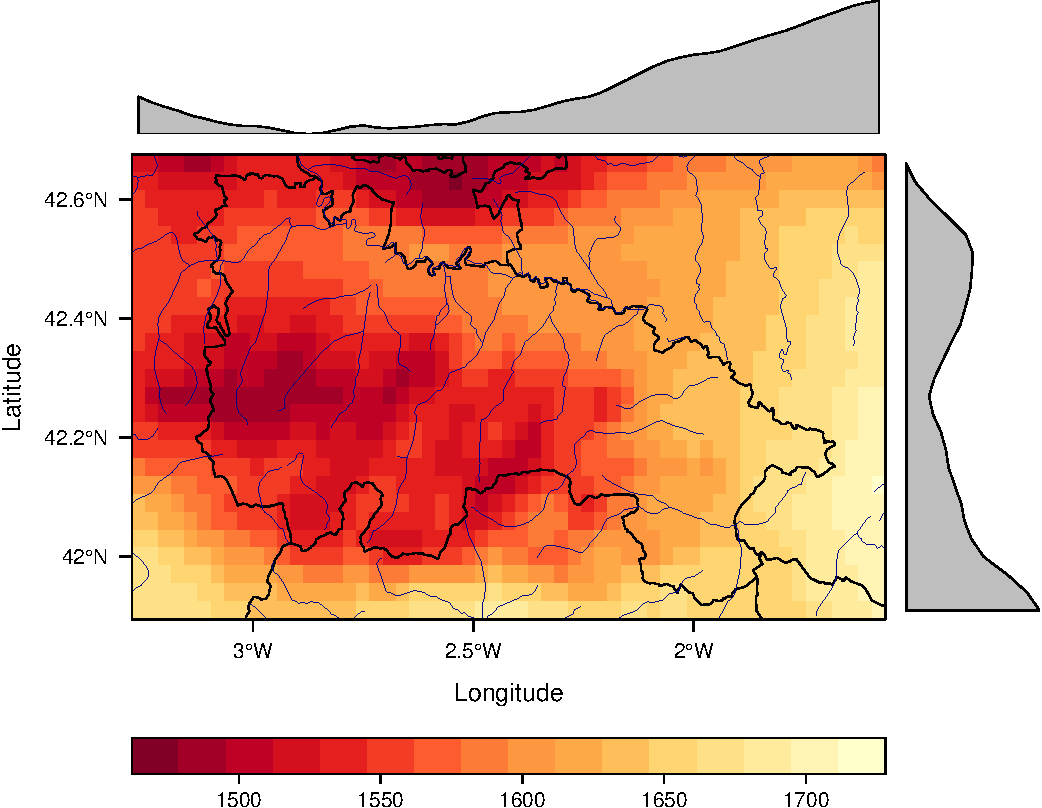
\includegraphics[width=\textwidth]{figs/GHI2005aCMSAF003x003.pdf}
  \caption{Annual GHI of 2005 from CM SAF estimates (0.03x0.03$^\circ$) in La Rioja}
  \label{fig:cmsaf}
\end{figure}

 \begin{figure}
    \centering
  
    \subfloat[Downscaling without
    KED]{\label{fig:noKEDdown}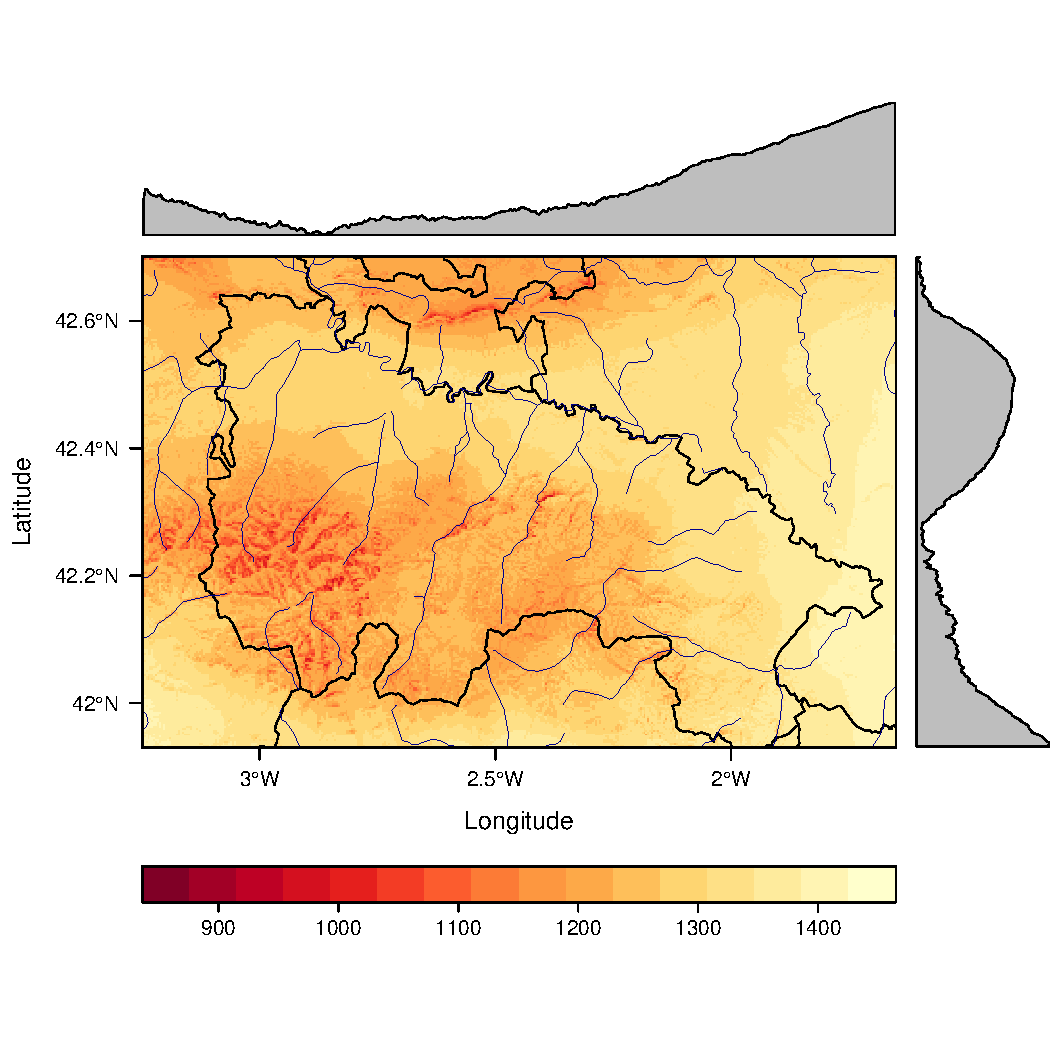
\includegraphics[height=0.45\textheight]{figs/GHI2005adownwithoutKED.pdf}}

    \subfloat[Downscaling with
    KED]{\label{fig:KED}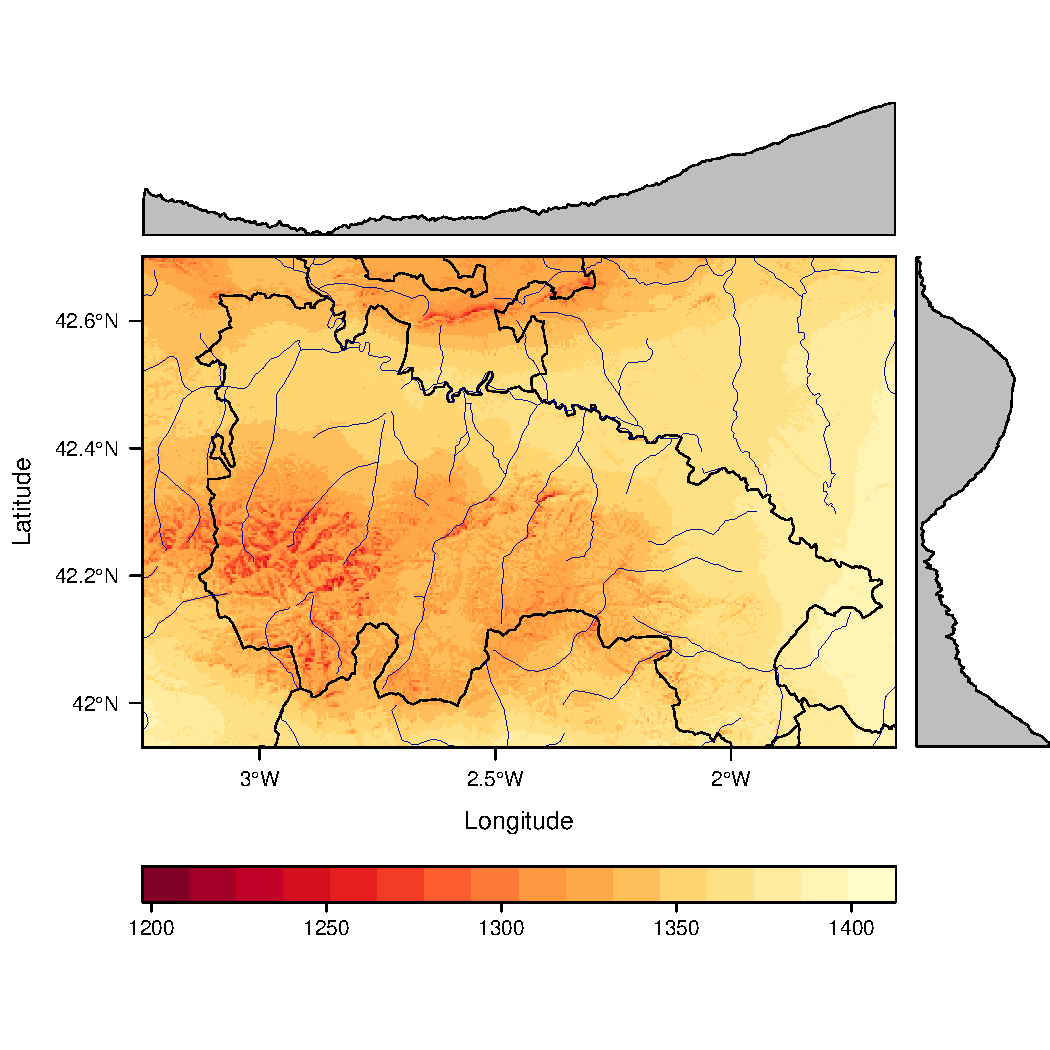
\includegraphics[height=0.45\textheight]{figs/GHI2005anual003x003.pdf}}
  
    \caption{Different estimations of global irradiation ($kWh/m^2$)}
    \label{fig:GHI}
\end{figure}


\begin{figure}
  \centering
  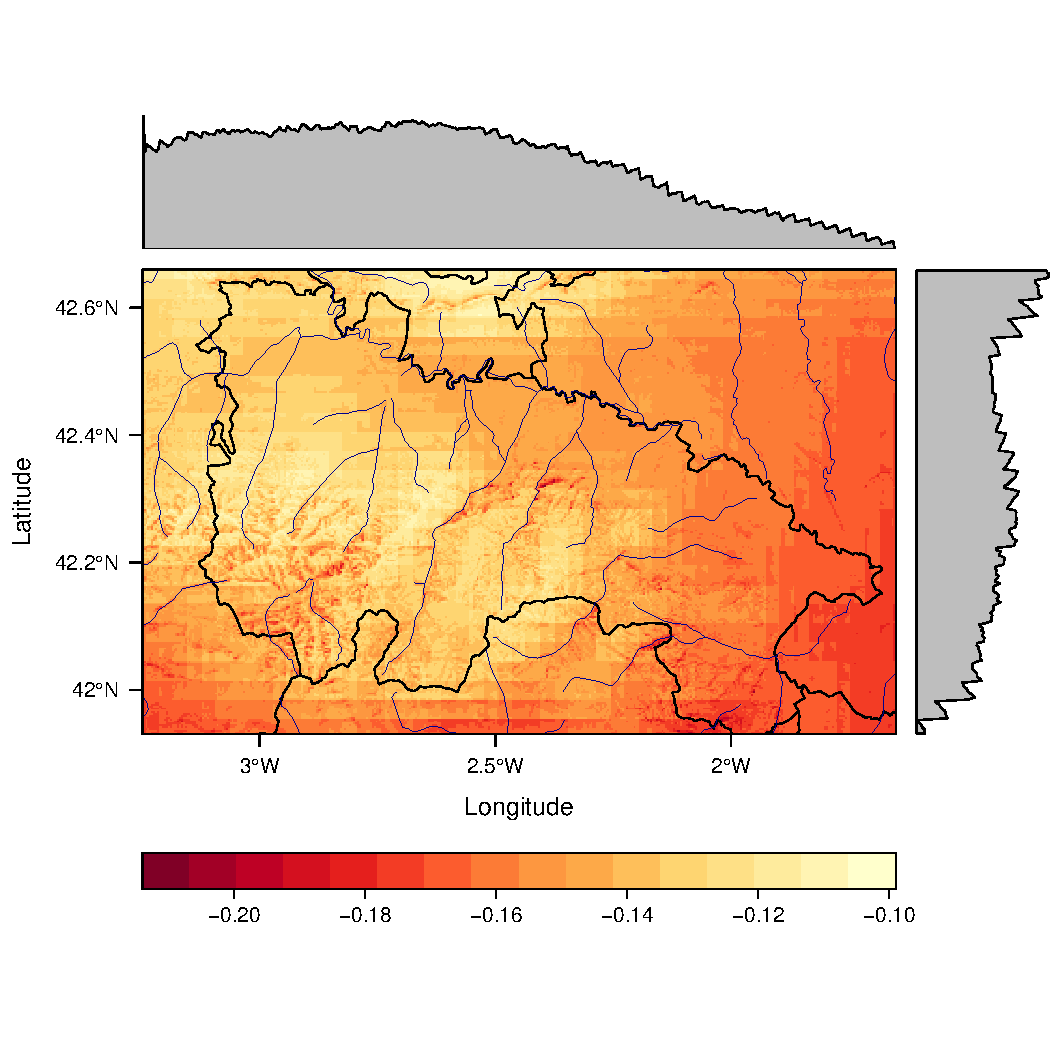
\includegraphics[width=\textwidth]{figs/diffwithKED.pdf}
  \caption{Relative difference of $GHI_{KED}$ and $GHI_{CMSAF, down}$  related to $GHI_{CMSAF, down}$}
  \label{fig:diffKEDcmsaf}
\end{figure}


The mean absolute error ($MAE$) is analyzed for the set of
stations (Figure~\ref{fig:mapstations}). Table~\ref{tab:MAE} shows
the improvement in errors when considering the KED in which a 14.03\% lower MAE is obtained when compared to the actual CM SAF. The
downscaling using KED presents lower MAE than with the original CM
SAF data. As it might be extracted from
Figures~\ref{fig:noKEDdown} and ~\ref{fig:cmsaf}, $GHI_{annual,
  down}$ is excesively lowered in certain regions of the area
studied compared to $GHI_{dis}$ and therefore its MAE
increases. However, considering the KED, the same trend in GHI reduction is considered and at the same time
estimates are closer to registered values from stations.

\begin{CodeChunk}
\begin{CodeInput}
R> G0yKrig_v <- extract(G0yKrig, UTM)

R> GHI2005a_v <- extract(GHIcmsaf, UTM)
R> SISa2005_v <- extract(SISa2005, UTM)

R> results <- (SISa2005_v, G0yKrig_v, GHI2005a_v)
R> MAE <- colMeans(abs(results - UTM$GHImed))n
R> names(MAE) <- c('MAEcmsaf', 'MAEkrig', 'MAEcmsafdown')
\end{CodeInput}
\end{CodeChunk}


\begin{table}[htb]
\caption{MAE of different scenarios against measured data from on-ground pyranometers ($kWh/m^2$)} \label{tab:MAE}
\begin{center}
\begin{tabular}{rrr}
 $MAE_{CM SAF}$  &  $MAE_{KED}$  &  $MAE_{CM SAF,down}$  \\
\hline
        119.6  &        102.9 &        175.6   \\
\end{tabular}
\end{center}
\end{table}


On the other hand, variability due to the downscaling procedure
can be considered with the \code{zonal} function from
\code{raster} package.

\begin{CodeChunk}
\begin{CodeInput}
R> cells <- raster(SISa2005dr)

R> xy <- as(SISa2005dr, 'SpatialPoints')
R> cells[] <- cellFromXY(SISa2005, xy)

R> SD <- SD2 <- raster(SISa2005)
R> SD[] <- zonal(G0yKrig, cells, sd)[,2]
R> SD2[] <- zonal(GHI2005a, cells, sd)[,2]
\end{CodeInput}
\end{CodeChunk}

Figures~\ref{fig:sdnoKED} and ~\ref{fig:sdKED} display the
standard deviations of the downscaled maps within each cell of the
original CM SAF raster (0.03x0.03$^\circ$). This \code{zonal} function leads to explain the intrinsecal variability of solar radiation within gross resolution pixels. As a result, in those pixels with higher standard deviation a higher variability will be present.  Figure~\ref{fig:zonal}
shows how the KED method smooth the deviation within pixels and
also the range of solar irradiation in the region
(Figures~\ref{fig:noKEDdown} and ~\ref{fig:KED}).

\begin{figure}
  \centering
  \subfloat[Downscaling without KED]{%
    \label{fig:sdnoKED}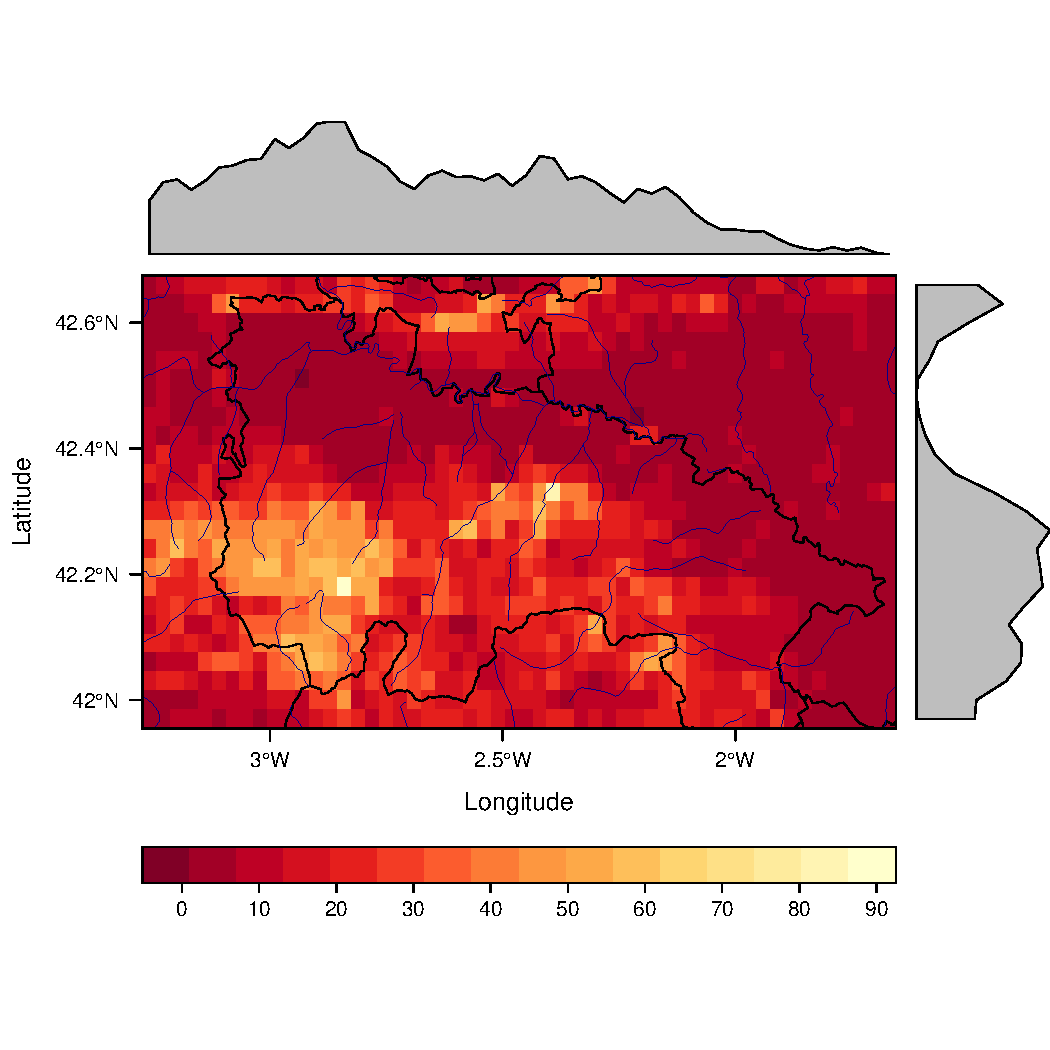
\includegraphics[height=0.45\textheight]{figs/sdwithoutKED.pdf}}

  \subfloat[Downscaling with KED]{%
    \label{fig:sdKED}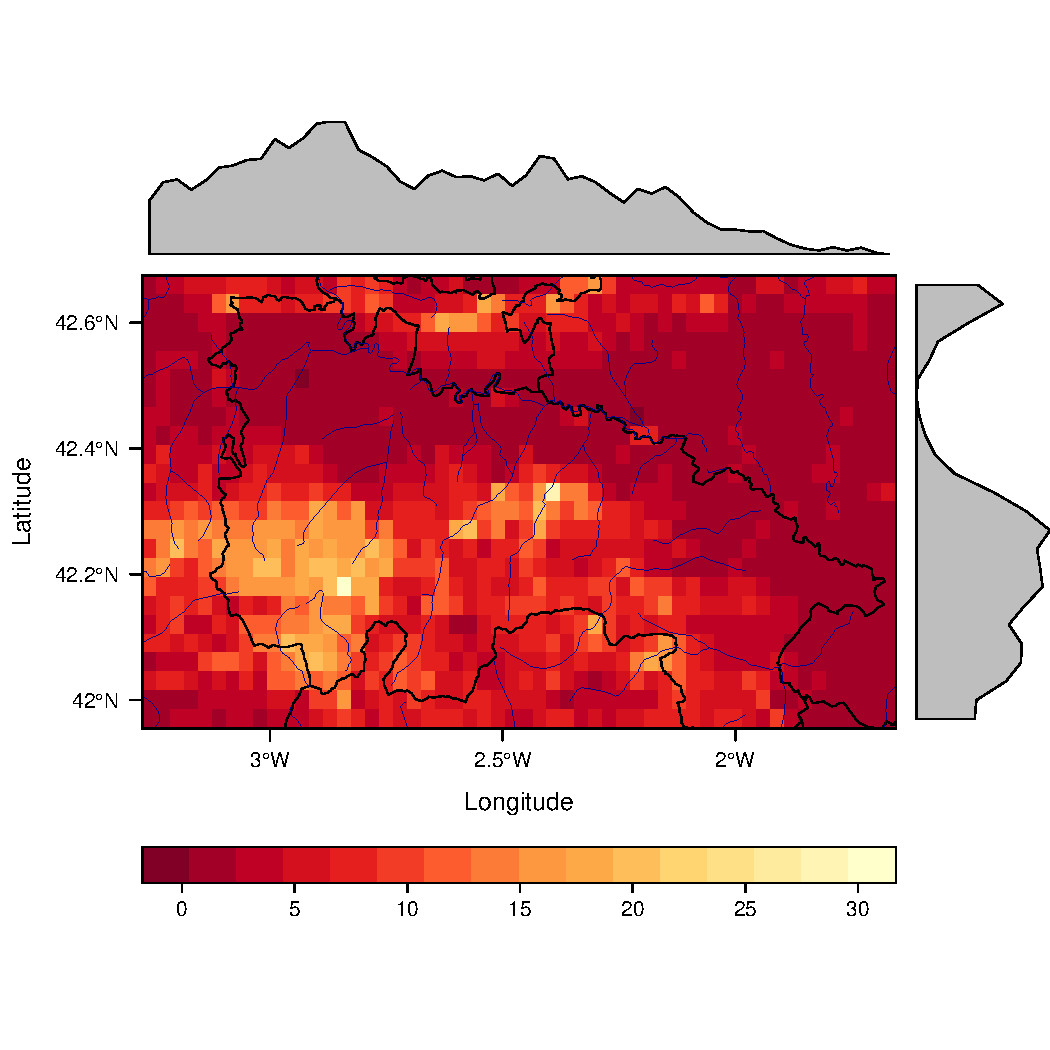
\includegraphics[height=0.45\textheight]{figs/sdKED.pdf}}
  \caption{Zonal standard deviations before and after the KED ($kWh/m^2$)}
  \label{fig:zonal}
\end{figure}

\section{Concluding comments}
A methodology to downscale solar irradiation is described and
presented using \proglang{R} software. This applied methodology is
useful to increase accuracy and spatial resolution of gross resolution
satellite-estimates of solar irradiation.

It has been proved that areas with complex topography present higher
differences with original gross resolution data as a consequence of
horizon blocking and lower sky-view factors and therefore, downscaling
is highly recommended in these areas.

\emph{Kriging with external drift} with \pkg{gstat} package has been
proved very useful in the downscaling of solar irradiation when some
on-ground registers are available and a explanatory variable is
provided.
  
This methodology has been implemented as an example within La Rioja
region in northern Spain, highlighting a mean absolute error 14\%
lower than with the original gross resolution database. The high
repeatibility of this methodology and the reduction in errors obtained might be also very useful in the
downscaling of other meteorological variables apart from solar
irradiation.

\section*{Session information}
\label{sec:session}

The results discussed in this paper were obtained in a session with
these characteristics:

\begin{itemize}\raggedright
  \item \proglang{R} version 2.15.2 (2012-10-26), \verb|x86_64-apple-darwin9.8.0|
  \item Locale: \verb|es_ES.UTF-8/es_ES.UTF-8/es_ES.UTF-8/C/es_ES.UTF-8/es_ES.UTF-8|
  \item Base packages: \pkg{base}, \pkg{datasets}, \pkg{graphics}, \pkg{grDevices}, \pkg{grid}, \pkg{methods}, \pkg{parallel}, \pkg{stats},\pkg{utils}
  \item Other packages: \pkg{foreign}~0.8-51, \pkg{gstat}~1.0-16, \pkg{hexbin}~1.26.0, \pkg{lattice}~0.20-15,
    \pkg{latticeExtra}~0.6-19, \pkg{maptools}~0.8-14, \pkg{raster}~2.1-16, \pkg{rasterVis}~0.20-01,
    \pkg{RColorBrewer}~1.0-5, \pkg{rgdal}~0.8-01, \pkg{solaR}~0.33, sp~1.0-8, \pkg{zoo}~1.7-9
  \item Loaded via a namespace (and not attached): \pkg{intervals}~0.14.0, \pkg{spacetime}~1.0-4,
    \pkg{tools}~2.15.2, \pkg{xts}~0.9-3
\end{itemize}


\section*{Acknowledgements}
We are indebted to the University of La Rioja (fellowship FPI 2012)
and the Research Institute of La Rioja ($IER$) for funding parts of
this research.


\bibliography{downscaling}


\end{document}

